\documentclass[12pt, openany, oneside]{book}

\usepackage{listings}
\usepackage[dvipsnames]{xcolor}
\usepackage{ctex}
\usepackage{fontspec}
\usepackage{setspace}
\usepackage{tikz}
\usepackage{anyfontsize}
\usepackage{sectsty}
\usepackage{titlesec}
\usepackage{float}
\usepackage[hidelinks]{hyperref}
\usepackage[a4paper]{geometry}
\usepackage{url}
\usepackage{amssymb}
\usepackage{fontawesome5}
\usepackage[most]{tcolorbox}
\usepackage{stackengine}
\usepackage{multirow}
\usepackage{makecell}
\usepackage[T1]{fontenc}
\usepackage{diagbox}
\usepackage{longtable}
\usepackage{newtxtt}
\usepackage{pgf-umlcd}
\usepackage{bbding}
\usepackage{amsmath}
\usepackage{tkz-graph}
\usepackage{drawstack}
\usepackage{dcolumn}
\usepackage{tikzpeople}

\usetikzlibrary{calc,positioning,arrows,fit,shapes}
\usetikzlibrary{shapes.multipart,chains}
\usetikzlibrary{shadows}
\usetikzlibrary{arrows.meta}
\usetikzlibrary{matrix,backgrounds}
\usetikzlibrary{automata}
\usetikzlibrary{scopes}

\tikzset{
	->,
	>=stealth,
	node distance=3cm,
	every state/.style={thick, fill=gray!10},
	initial text=$ Start $,
}

\tikzset{block/.style={
        font=\sffamily,
        draw=black,
        thin,
        fill=pink!50,
        rectangle split,
        rectangle split horizontal,
        rectangle split parts=#1,
        outer sep=0pt},
        gblock/.style={
            block,
            rectangle split parts=#1,
            fill=green!30}
        }

\makeatletter
\newcommand{\verbatimfont}[1]{\renewcommand{\verbatim@font}{\ttfamily#1}}
\makeatother

\makeatletter
\def\BState{\State\hskip-\ALG@thistlm}
\makeatother

\def\rlwd{.5pt} \def\rlht{2.2ex} \def\rldp{.5ex}
\def\mydiv#1{~
  \rule[-\rldp]{\rlwd}{\rlht}
  \setbox0=\hbox{~#1}
  \stackunder[\dimexpr\rldp-\rlwd]{~#1}{\rule{\wd0}{\rlwd}}
}

\definecolor{mycolor}{RGB}{0,128,128}
\newtcbox{\mybox} {
    on line,
    colback=mycolor,
    fontupper=\bfseries\color{white},
    boxrule=0pt,
    arc=5pt, 
    boxsep=0pt, 
    left=2pt, 
    right=2pt, 
    top=5pt, 
    bottom=5pt
}

\setstretch{1.5}
\setlength{\parindent}{0cm}

\geometry{a4paper,top=2.5cm,bottom=2.5cm}

\titleformat{\chapter}{\Huge\Huge\bfseries}{\chaptertitlename\ \thechapter{\ }}{0pt}{\Huge}{}
\titlespacing{\chapter}{0pt}{0pt}{12pt}

\definecolor{dkgreen}{rgb}{0,0.4,0}
\definecolor{gray}{rgb}{0.5,0.5,0.5}
\definecolor{mauve}{rgb}{0.58,0,0.82}
\definecolor{LightGray}{gray}{0.9}

\lstset{
    basicstyle=\linespread{1.3} \fontspec{Consolas},    %  the size of the fonts that are used for the code
	basewidth=0.5em,
    numbers=left,            % where to put the line-numbers
    numberstyle=\color{black},  % the style that is used for the line-numbers
    numbersep=10pt,                  % how far the line-numbers are from the code
    backgroundcolor=\color{white},
    showspaces=false,
    showstringspaces=false,
    showtabs=false,
    frame=single,                   % adds a frame around the code
    rulecolor=\color{black},        % if not set, the frame-color may be changed on line-breaks within not-black text (e.g. commens (green here))
    tabsize=4,                      % sets default tabsize to 2 spaces
    captionpos=t,                   % sets the caption-position to bottom
    breaklines=false,                % sets automatic line breaking
    breakatwhitespace=true,        % sets if automatic breaks should only happen at whitespace
    title=\lstname,                   % show the filename of files included with \lstinputlisting;
    % also try caption instead of title
    numberstyle=\color{black},		% line number color
    keywordstyle=\color{blue},          % keyword style
    commentstyle=\color{dkgreen},       % comment style
    stringstyle=\color{mauve},         % string literal style
    escapeinside={\%*}{*)},            % if you want to add LaTeX within your code
    morekeywords={*,...}               % if you want to add more keywords to the set
}

\begin{document}

\thispagestyle{empty}

\begin{tikzpicture}[overlay,remember picture]
	\fill[
		black!2]
	(current page.south west) rectangle (current page.north east);

	\shade[
		left color=Dandelion,
		right color=Dandelion!40,
		transform canvas ={rotate around ={45:($(current page.north west)+(0,-6)$)}}]
	($(current page.north west)+(0,-6)$) rectangle ++(9,1.5);

	\shade[
		left color=lightgray,
		right color=lightgray!50,
		rounded corners=0.75cm,
		transform canvas ={rotate around ={45:($(current page.north west)+(.5,-10)$)}}]
	($(current page.north west)+(0.5,-10)$) rectangle ++(15,1.5);

	\shade[
		left color=lightgray,
		rounded corners=0.3cm,
		transform canvas ={rotate around ={45:($(current page.north west)+(.5,-10)$)}}] ($(current page.north west)+(1.5,-9.55)$) rectangle ++(7,.6);

	\shade[
		left color=orange!80,
		right color=orange!60,
		rounded corners=0.4cm,
		transform canvas ={rotate around ={45:($(current page.north)+(-1.5,-3)$)}}]
	($(current page.north)+(-1.5,-3)$) rectangle ++(9,0.8);

	\shade[
		left color=red!80,
		right color=red!80,
		rounded corners=0.9cm,
		transform canvas ={rotate around ={45:($(current page.north)+(-3,-8)$)}}] ($(current page.north)+(-3,-8)$) rectangle ++(15,1.8);

	\shade[
		left color=orange,
		right color=Dandelion,
		rounded corners=0.9cm,
		transform canvas ={rotate around ={45:($(current page.north west)+(4,-15.5)$)}}]
	($(current page.north west)+(4,-15.5)$) rectangle ++(30,1.8);

	\shade[
		left color=RoyalBlue,
		right color=Emerald,
		rounded corners=0.75cm,
		transform canvas ={rotate around ={45:($(current page.north west)+(13,-10)$)}}]
	($(current page.north west)+(13,-10)$) rectangle ++(15,1.5);

	\shade[
		left color=lightgray,
		rounded corners=0.3cm,
		transform canvas ={rotate around ={45:($(current page.north west)+(18,-8)$)}}]
	($(current page.north west)+(18,-8)$) rectangle ++(15,0.6);

	\shade[
		left color=lightgray,
		rounded corners=0.4cm,
		transform canvas ={rotate around ={45:($(current page.north west)+(19,-5.65)$)}}]
	($(current page.north west)+(19,-5.65)$) rectangle ++(15,0.8);

	\shade[
		left color=OrangeRed,
		right color=red!80,
		rounded corners=0.6cm,
		transform canvas ={rotate around ={45:($(current page.north west)+(20,-9)$)}}]
	($(current page.north west)+(20,-9)$) rectangle ++(14,1.2);

	% Title
	\node[align=center] at ($(current page.center)+(0,-7)$)
	{
	{\fontsize{60}{60} \selectfont {{编译原理}}}\\[1cm]
	{\fontsize{40}{40} \selectfont {{Compilers}}}\\[2cm]
	{\fontsize{20}{19.2} \selectfont \textcolor{orange}{ \bf 极夜酱}}\\[4pt]
	};
\end{tikzpicture}

\newpage

\pagestyle{plain}
\setcounter{page}{1}
\setcounter{tocdepth}{1}
\tableofcontents

\newpage

\setcounter{page}{1}

\chapter{有限状态自动机}

\section{字母表}

\subsection{字母表(Alphabet)}

字母表是一个非空的有限集合,一般用$ \Sigma $表示,集合中的元素被称为符号/字符(symbol)。\\

例如:

\begin{itemize}
	\item $ \Sigma = \{0, 1\} $:二进制数集合。
	\item $ \Sigma = \{a, b, \cdots, z\} $:小写字母集合。
	\item $ \Sigma = \{(, ), [, ], \{, \}\} $:括号集合。
\end{itemize}

\vspace{0.5cm}

\subsection{串(String)}

串是一个由字母表中的字符组成的有限序列。\\

例如:

\begin{itemize}
	\item 0011和11是$ \Sigma = \{0, 1\} $上的串。
	\item abc和bbb是$ \Sigma = \{a, b, \cdots, z\} $上的串。
	\item (())和(()是$ \Sigma = \{(, ), [, ], \{, \}\} $上的串。
\end{itemize}

\vspace{0.5cm}

\subsubsection{空串}

空串使用$ \epsilon $表示。\\

\subsubsection{串的长度}

\begin{itemize}
	\item $ |0010| = 4 $
	\item $ |aa| = 2 $
	\item $ |\epsilon| = 0 $
\end{itemize}

\vspace{0.5cm}

\subsubsection{前缀(prefix)}

\begin{itemize}
	\item aa是aaabc的前缀
	\item aaab是aaabc的前缀
	\item aaabc是aaabc的前缀
\end{itemize}

\vspace{0.5cm}

\subsubsection{后缀(suffix)}

\begin{itemize}
	\item bc是aaabc的后缀
	\item abc是aaabc的后缀
	\item aaabc是aaabc的后缀
\end{itemize}

\vspace{0.5cm}

\subsubsection{子串(substring)}

\begin{itemize}
	\item ab是aaabc的子串
	\item aaa是aaabc的子串
	\item aaabc是aaabc的子串
\end{itemize}

\vspace{0.5cm}

\subsubsection{连接(concatenation)}

当$ \omega = abd $,$ \alpha = ce $,那么$ \omega\alpha = abdce $。\\

\subsubsection{指数(exponentiation)}

当$ \omega = abd $,那么$ \omega^3 = abdabdabd $,$ \omega^0 = \epsilon $。\\

\subsubsection{反转(reversal)}

当$ \omega = abd $,那么$ \omega^R = dba $。\\

\subsection{克林闭包(Kleene Closure)}

$ \Sigma^k $用于表示所有在字母表$ \Sigma $上的长度为$ k $的串的集合。\\

例如,$ \Sigma = \{a, b\} $,那么$ \Sigma^2 = \{ab, ba, aa, bb\} $,$ \Sigma^0 = \{\epsilon\} $。\\

克林闭包$ \Sigma^* $用于表示所有在字母表$ \Sigma $上能够组成的串的集合。\\

\vspace{-1cm}

\begin{align}
	\Sigma^* = \Sigma^0 \cup \Sigma^1 \cup \Sigma^2 \cup \cdots = \bigcup_{k \ge 0}\Sigma^k
\end{align}

正闭包$ \Sigma^+ $则是在$ \Sigma^* $中除了空串以外的所有串的集合。\\

\vspace{-1cm}

\begin{align}
	\Sigma^+ = \Sigma^1 \cup \Sigma^2 \cup \Sigma^3 \cup \cdots = \bigcup_{k > 0}\Sigma^k
\end{align}

\newpage

\section{语言}

\subsection{语言(Language)}

语言是一个字母表中所构成串的集合。\\

例如,$ \Sigma = \{a, b, c, \cdots, z\} $,那么所有英语单词所构成的集合$ L $就是字母表$ \Sigma $上的语言。\\

假设$ A = \{good, bad\} $和$ B = \{boy, girl\} $是两个语言,语言之间可以进行以下操作。\\

\subsubsection{并集(union)}

\vspace{-1cm}

\begin{align}
	A \cup B = \{x\ |\ x \in A \text{ or } x \in B\}
\end{align}

$ A \cup B = \{good, bad, boy, girl\} $\\

\subsubsection{连接(concatenation)}

\vspace{-1cm}

\begin{align}
	A \circ B = \{xy\ |\ x \in A \text{ or } y \in B\}
\end{align}

$ A \circ B = \{goodboy, goodgirl, badboy, badgirl\} $\\

\subsubsection{闭包}

\vspace{-1cm}

\begin{align}
	A^* = \{x_1, x_2, \cdots, x_k\ |\ k \ge 0 \text{ and each } x_i \in A\}
\end{align}

$ A^* = \{\epsilon, good, bad, goodgood, goodbad, badgood, badbad, goodgoodgood, goodgoodbad, \cdots\} $\\

语法和语言与自动机理论密切相关,它们是许多软件实现的基础,例如编译器/解释器、文本编辑器、文本搜索、系统验证等。\\

在自动机理论中,要处理的问题就是判断一个给定的串是否属于某个语言。\\

例如:

\begin{itemize}
	\item $ 0^*10^* $: 只包含一个1的串的集合。

	\item $ \Sigma^*1\Sigma^* $:至少有一个1的串的集合。

	\item $ \Sigma^*001\Sigma^* $:包含子串001的串的集合。

	\item $ (\Sigma\Sigma)^* $:长度为偶数的串的集合。

	\item $ (\Sigma\Sigma\Sigma)^* $:长度为3的倍数的串的集合。
\end{itemize}

\newpage

\section{DFA}

\subsection{DFA(Deterministic Finite Automaton)}

有限状态机(FSM, Finite State Machine)用于决定程序当前状态和状态间的切换,状态机最终只能指向一个结果。

\begin{figure}[H]
	\centering
	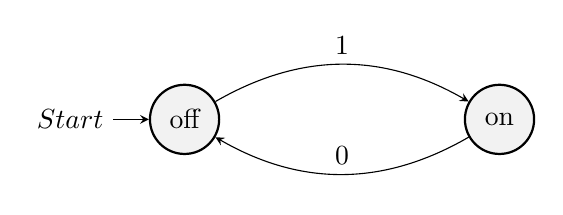
\begin{tikzpicture}[node distance=4cm]
		\node[state, initial, draw, align=center] (s1) {off};
		\node[state, right of=s1, draw, align=center] (s2) {on};

		\draw[->] (s1) edge[above, bend left] node{1} (s2);
		\draw[->] (s2) edge[above, bend left] node{0} (s1);
	\end{tikzpicture}
	\caption{有限状态机}
\end{figure}

确定性有限状态自动机DFA使用一个五元组$ (Q, \Sigma, \delta, q_0, F) $表示,其中

\begin{itemize}
	\item $ Q $:状态的集合
	\item $ \Sigma $:字母表
	\item $ \delta $:状态转移函数(transition function)
	\item $ q_0 $:初始状态
	\item $ F $:终结状态集合
\end{itemize}

例如DFA可以用来识别空串或者以0结尾的串:

\begin{figure}[H]
	\centering
	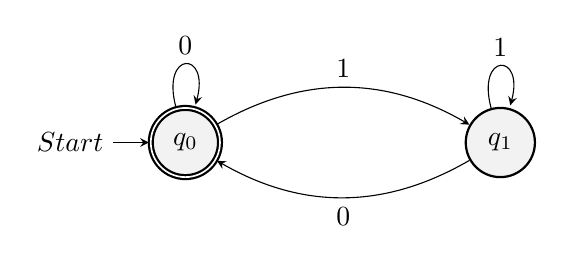
\begin{tikzpicture}
		\node[state, initial, accepting] (q0) {$ q_0 $};
		\node[state] (q1) at (4,0) {$ q_1 $};

		\draw (q0) edge[loop above] node{0} (q0)
		(q0) edge[bend left, above] node{1} (q1)
		(q1) edge[bend left, below] node{0} (q0)
		(q1) edge[loop above] node{1} (q1);
	\end{tikzpicture}
\end{figure}

其中$ Q = \{q_0, q_1\} $,$ \Sigma = \{0, 1\} $,$ q_0 $为初始状态,$ F = \{q_0\} $,$ \delta $为

\begin{table}[H]
	\center
	\begin{tabular}{|c|c|c|}
		\hline
		\multicolumn{1}{|c|}{\multirow{2}{*}{状态}} & \multicolumn{2}{c|}{输入}           \\ \cline{2-3}
		                                            & 0                         & 1       \\
		\hline
		$ q_0 $                                     & $ q_0 $                   & $ q_1 $ \\
		\hline
		$ q_1 $                                     & $ q_0 $                   & $ q_1 $ \\
		\hline
	\end{tabular}
\end{table}

能够被有限自动机接受的语言被称为正则语言(regular language)。\\

例如,构建一个能够识别所有包含子串001的串的DFA:

\begin{figure}[H]
	\centering
	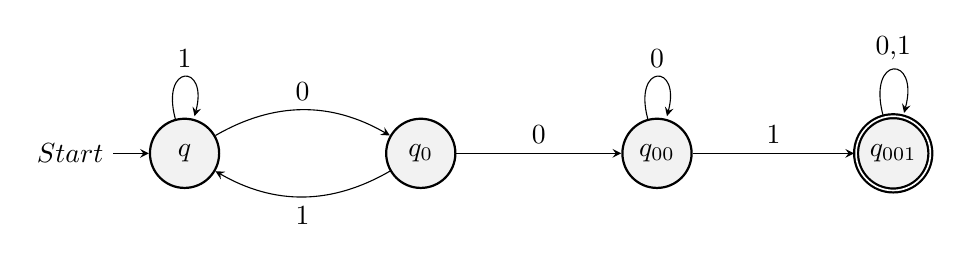
\begin{tikzpicture}
		\node[state, initial] (q) {$ q $};
		\node[state] (q0) at (3,0) {$ q_0 $};
		\node[state] (q00) at (6,0) {$ q_{00} $};
		\node[state, accepting] (q001) at (9,0) {$ q_{001} $};

		\draw (q) edge[loop above] node{1} (q)
		(q) edge[bend left, above] node{0} (q0)
		(q0) edge[bend left, below] node{1} (q)
		(q0) edge[above] node{0} (q00)
		(q00) edge[loop above] node{0} (q00)
		(q00) edge[above] node{1} (q001)
		(q001) edge[loop above] node{0,1} (q001);
	\end{tikzpicture}
\end{figure}

\vspace{0.5cm}

\subsection{最小化DFA}

有限状态机的最小化,即将一个有限状态机转换为一个更小的有限状态机,使得状态的数目最少。\\

对于两个状态,如果它们之间的转移函数相同,则这两个状态可以合并为一个状态。

\begin{figure}[H]
	\centering
	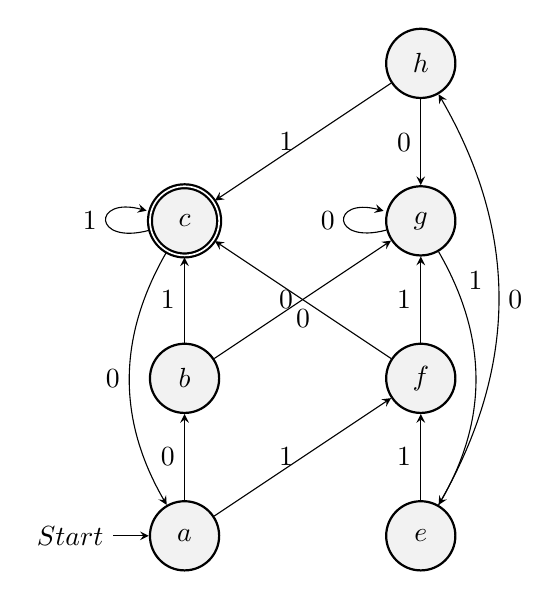
\begin{tikzpicture}
		\node[state, initial] (a) {$ a $};
		\node[state] (b) at (0,2) {$ b $};
		\node[state, accepting] (c) at (0,4) {$ c $};
		\node[state] (e) at (3,0) {$ e $};
		\node[state] (f) at (3,2) {$ f $};
		\node[state] (g) at (3,4) {$ g $};
		\node[state] (h) at (3,6) {$ h $};

		\draw (a) edge[left] node{0} (b)
		(a) edge[left] node{1} (f)
		(b) edge[left] node{1} (c)
		(b) edge[left] node{0} (g)
		(c) edge[bend right, left] node{0} (a)
		(c) edge[loop left] node{1} (c)
		(e) edge[bend right, right] node{0} (h)
		(e) edge[left] node{1} (f)
		(f) edge[below] node{0} (c)
		(f) edge[left] node{1} (g)
		(g) edge[loop left] node{0} (g)
		(g) edge[bend left, above] node[yshift=1cm]{1} (e)
		(h) edge[left] node{0} (g)
		(h) edge[left] node{1} (c);
	\end{tikzpicture}
\end{figure}

在这个DFA中,状态$ b $和$ h $是等价的,当接收0时都转移到状态$ g $,当接收1时都转移到状态$ c $。同时状态$ a $和$ e $也是等价的,状态$ a $接收0转移到状态$ b $,状态$ e $接收0转移到状态$ h $,状态$ a $和$ e $接收1时都转移到状态$ f $。\\

因此,状态$ b $和$ h $以及状态$ a $和$ e $可以进行合并。

\begin{figure}[H]
	\centering
	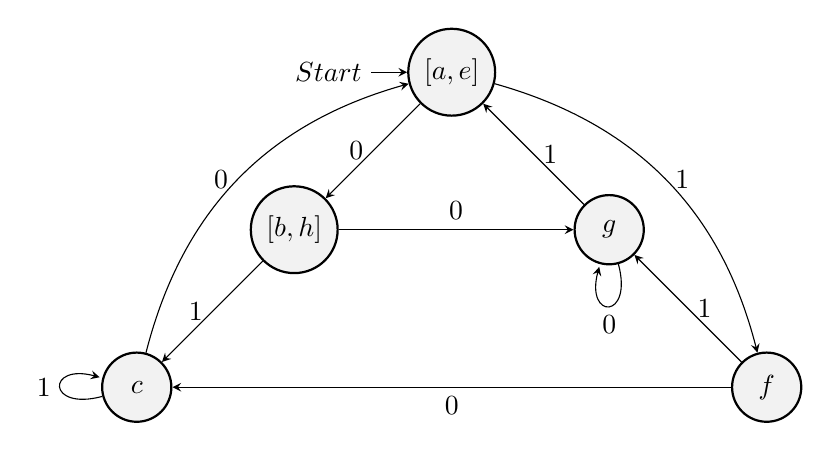
\begin{tikzpicture}
		\node[state, initial] (ae) {$ [a, e] $};
		\node[state] (bh) at (-2,-2) {$ [b, h] $};
		\node[state] (g) at (2,-2) {$ g $};
		\node[state] (c) at (-4,-4) {$ c $};
		\node[state] (f) at (4,-4) {$ f $};

		\draw (ae) edge[left] node{0} (bh)
		(ae) edge[bend left, right] node{1} (f)
		(bh) edge[above] node{0} (g)
		(bh) edge[left] node{1} (c)
		(c) edge[loop left] node{1} (c)
		(c) edge[bend left, left] node{0} (ae)
		(g) edge[right] node{1} (ae)
		(g) edge[loop below] node{0} (g)
		(f) edge[right] node{1} (g)
		(f) edge[below] node{0} (c);
	\end{tikzpicture}
\end{figure}

\newpage

\section{NFA}

\subsection{NFA(Non-deterministic Finite Automaton)}

在DFA中,每个状态的下一个状态都是唯一确定的,但是非确定性有限状态自动机NFA可能会存在多个下一状态。\\

例如在这个NFA中,状态$ q_0 $存在两个接收1的箭头,而状态$ q_1 $没有接收1的箭头。

\begin{figure}[H]
	\centering
	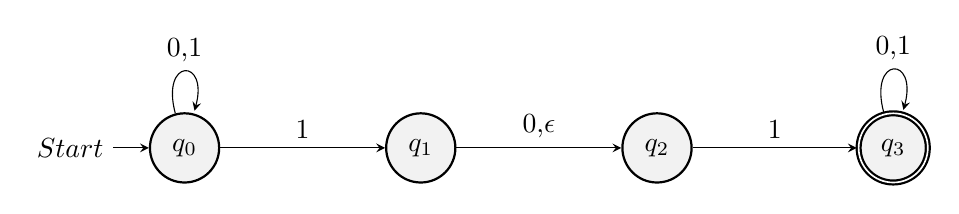
\begin{tikzpicture}
		\node[state, initial] (q0) {$ q_0 $};
		\node[state] (q1) at (3,0) {$ q_1 $};
		\node[state] (q2) at (6,0) {$ q_2 $};
		\node[state, accepting] (q3) at (9,0) {$ q_3 $};

		\draw (q0) edge[above] node{1} (q1)
		(q0) edge[loop above] node{0,1} (q0)
		(q1) edge[above] node{0,$ \epsilon $} (q2)
		(q2) edge[above] node{1} (q3)
		(q3) edge[loop above] node{0,1} (q3);
	\end{tikzpicture}
\end{figure}

因此,在NFA中,每个状态允许对相同输入存在0个、1个或多个转移的状态。如果存在一条能够到达终结状态的路径,那么就称当前的输入是被NFA接受的。\\

\subsection{DFA与NFA的转换}

NFA并不比DFA更加强大,理论证明NFA与DFA是等价的。\\

例如将一个NFA转换为DFA:

\begin{figure}[H]
	\centering
	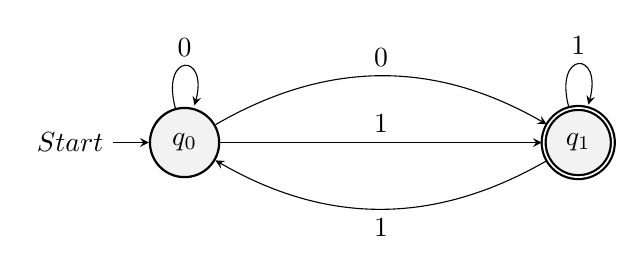
\begin{tikzpicture}
		\node[state, initial] (q0) {$ q_0 $};
		\node[state, accepting] (q1) at (5,0) {$ q_1 $};

		\draw (q0) edge[loop above] node{0} (q0)
		(q0) edge[bend left, above] node{0} (q1)
		(q0) edge[above] node{1} (q1)
		(q1) edge[bend left, below] node{1} (q0)
		(q1) edge[loop above] node{1} (q1);
	\end{tikzpicture}
\end{figure}

构建一个与NFA等价的DFA,只需将NFA中转换到的状态集合作为DFA中的一个状态即可。

\begin{figure}[H]
	\centering
	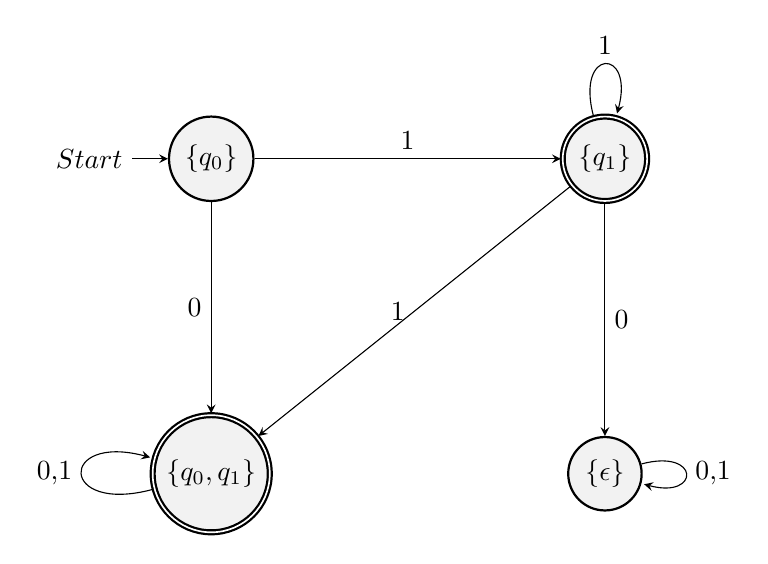
\begin{tikzpicture}
		\node[state, initial] (q0) {$ \{q_0\} $};
		\node[state, accepting] (q1) at (5,0) {$ \{q_1\} $};
		\node[state, accepting] (q0q1) at (0,-4) {$ \{q_0, q_1\} $};
		\node[state] (e) at (5,-4) {$ \{\epsilon\} $};

		\draw (q0) edge[left] node{0} (q0q1)
		(q0) edge[above] node{1} (q1)
		(q1) edge[loop above] node{1} (q1)
		(q1) edge[left] node{1} (q0q1)
		(q1) edge[right] node{0} (e)
		(q0q1) edge[loop left] node{0,1} (q0q1)
		(e) edge[loop right] node{0,1} (e);
	\end{tikzpicture}
\end{figure}

\vspace{0.5cm}

\subsection{$ \epsilon $-NFA}

$ \epsilon $-NFA允许不消耗输入字符在状态之间转移。\\

例如以下$ \epsilon $-NFA能够接受小数,如+3.14、-0.12、.71、2.等。

\begin{figure}[H]
	\centering
	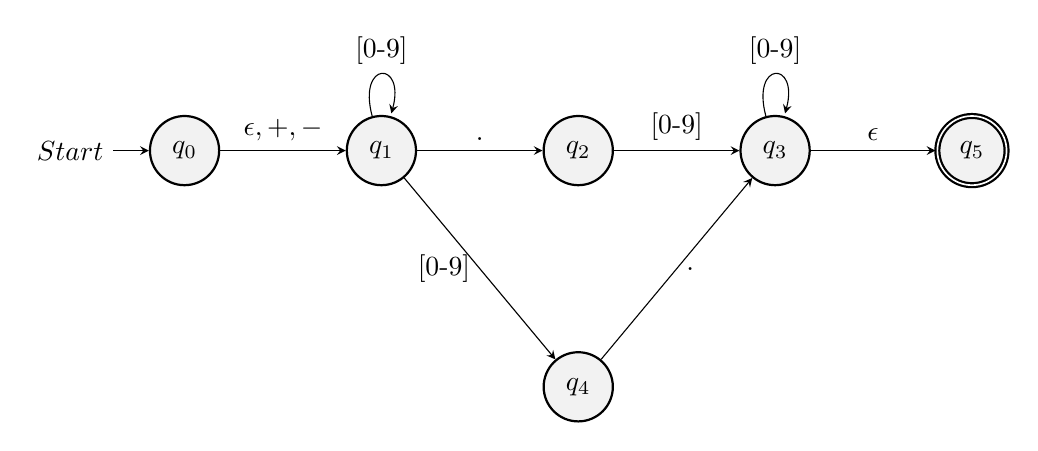
\begin{tikzpicture}
		\node[state, initial] (q0) {$ q_0 $};
		\node[state] (q1) at (2.5,0) {$ q_1 $};
		\node[state] (q2) at (5,0) {$ q_2 $};
		\node[state] (q3) at (7.5,0) {$ q_3 $};
		\node[state] (q4) at (5,-3) {$ q_4 $};
		\node[state, accepting] (q5) at (10,0) {$ q_5 $};

		\draw (q0) edge[above] node{$ \epsilon, +, - $} (q1)
		(q1) edge[loop above] node{[0-9]} (q1)
		(q1) edge[above] node{.} (q2)
		(q1) edge[left] node{[0-9]} (q4)
		(q2) edge[above] node{[0-9]} (q3)
		(q3) edge[loop above] node{[0-9]} (q3)
		(q4) edge[right] node{.} (q3)
		(q3) edge[above] node{$ \epsilon $} (q5);
	\end{tikzpicture}
\end{figure}

\newpage

\section{正则表达式}

\subsection{编译器(Compiler)}

编译器是一种特殊的程序,可以将一种编程语言的源代码翻译成机器码、字节码或另一种编程语言。\\

编译器包含以下阶段:

\begin{enumerate}
	\item 词法分析器(lexical analyzer)
	\item 语法分析器(syntex analyzer)
	\item 语义分析器(semantic analyzer)
	\item 中间代码生成器(intermediate code generator)
	\item 代码优化器(code optimizer)
	\item 代码生成器(code generator)
\end{enumerate}

\vspace{0.5cm}

\subsection{词法分析}

词法分析是编译器的第一步,它的主要任务是读取源代码,并生成能够被解析器(parser)进行语法分析的tokens和语法书(syntex tree)。\\

例如time = hour * 60 + minute,经过词法分析后,将会得到:

\begin{itemize}
	\item id(time)
	\item assignment(=)
	\item id(hour)
	\item op(*)
	\item num(60)
	\item op(+)
	\item id(minute)
\end{itemize}

\begin{figure}[H]
	\centering
	\begin{tikzpicture}[
			-,
			level distance=2cm,
			level 1/.style={sibling distance=5cm},
			level 2/.style={sibling distance=3cm},
			level 3/.style={sibling distance=3cm}
		]
		\node {assignment(=)}
		child {
				node {id(time)}
			}
		child {
				node {op(+)}
				child {
						node {op(*)}
						child {
								node {id(hour)}
							}
						child {
								node {num(60)}
							}
					}
				child {
						node {minute}
					}
			};
	\end{tikzpicture}
	\caption{语法树}
\end{figure}

\vspace{0.5cm}

\subsection{正则表达式(Regex, Regular Expression)}

正则表达式描述了字符串匹配的模式(pattern),可以用来检查一个串是否包含某个子串、替换子串、或提取符合条件的子串。像grep、vi、python、lex等工具都支持正则表达式的使用。\\

例如用于匹配一个合法的变量名的正则表达式为[a-zA-Z\_][a-zA-Z0-9\_]*。即变量名只能由字母或下划线开头,后面可以是任意多个字母、数字或下划线。\\

正则表达式支持以下操作:

\begin{itemize}
	\item 连接:$ ab $或$ a \cdot b $
	\item 选择:$ a\ |\ b $
	\item 克林闭包:$ a^* = \{\epsilon, a, aa, aaa, \cdots\} $
	\item 匹配至少1次:$ a^+ = aa^* $
	\item 匹配0次或1次:$ a? = a\ |\ \epsilon $
	\item 匹配任意字符:$ . $
	\item 补集:$ ~(a\ |\ b) $
\end{itemize}

其中克林闭包运算的优先级最高,其次是连接,最后是选择。\\

例如$ (a\ |\ b)^*aa(a\ |\ b)^* $用于匹配包含连续的a的串,$ b^*(abb^*)^*(a\ |\ \epsilon) $用于匹配没有连续的a的串。\\

然而$ a^nb^n\ (n \ge 0) $却不是正则语言,因为它无法用有限个状态来验证a和b的出现次数是相等的。\\

\newpage
\chapter{上下文无关语言}

\section{上下文无关文法}

\subsection{上下文无关文法(CFG, Context Free Grammar)}

CFG能够描述某些具有递归结构的特征,它有足够强的语言表达力来表示大多数编程语言的语法。\\

CFG由一个四元组$ (V, T, P, S) $表示:

\begin{itemize}
    \item $ V $:变元(variable)/非终结符(non-terminal)集合,用大写字母表示。
    \item $ T $:终结符(terminal)集合,用小写字母表示。
    \item $ P $:产生式(production)集合。
    \item $ S $:开始符号。
\end{itemize}

\vspace{0.5cm}

一个文法由一组替换规则产生。产生式集合

\vspace{-1cm}

\begin{align*}
    A & \rightarrow \alpha_1 \\
    A & \rightarrow \alpha_2 \\
      & \cdots               \\
    A & \rightarrow \alpha_k
\end{align*}

可以被写成$ A \rightarrow \alpha_1\ |\ \alpha_2\ |\ \cdots\ |\ \alpha_k\ $的形式。\\

\subsection{推导(Derivation)}

推导用于确定符合文法规则的串的集合,即用来确定一个语言。\\

推导从开始符号开始,通过产生式进行替换,得到最终结果。\\

例如$ E \rightarrow E + E\ |\ E * E\ |\ (E)\ |\ id $,由开始符号$ E $可以推导出$ (id + id) * id $。

\vspace{-1cm}

\begin{align*}
    E & \Rightarrow E * E          \\
      & \Rightarrow (E) * E        \\
      & \Rightarrow (E) * id       \\
      & \Rightarrow (E + E) * id   \\
      & \Rightarrow (E + id) * id  \\
      & \Rightarrow (id + id) * id
\end{align*}

解析树(parse tree)是描述推导的一种直观方法。\\

\begin{figure}[H]
    \centering
    \begin{tikzpicture}[
            -,
            level distance=1.5cm,
            level 1/.style={sibling distance=4cm},
            level 2/.style={sibling distance=3cm},
            level 3/.style={sibling distance=2cm},
            level 4/.style={sibling distance=1cm}
        ]
        \node {$ E $}
        child {
                node {$ E $}
                child {
                        node {$ ( $}
                    }
                child {
                        node {$ E $}
                        child {
                                node {$ E $}
                                child {
                                        node {$ id $}
                                    }
                            }
                        child {
                                node {$ + $}
                            }
                        child {
                                node {$ E $}
                                child {
                                        node {$ id $}
                                    }
                            }
                    }
                child {
                        node {$ ) $}
                    }
            }
        child {
                node {$ * $}
            }
        child {
                node {$ E $}
                child {
                        node {$ id $}
                    }
            };
    \end{tikzpicture}
    \caption{分析树}
\end{figure}

\vspace{0.5cm}

如果只关注语义分析和代码生成所需的信息,可以将分析树简化为一棵抽象语法树(abstract syntex tree)。\\

\begin{figure}[H]
    \centering
    \begin{tikzpicture}[
            -,
            level distance=1.5cm,
            level 1/.style={sibling distance=3cm},
            level 2/.style={sibling distance=2cm},
            level 3/.style={sibling distance=2cm}
        ]
        \node {$ * $}
        child {
                node {$ + $}
                child {
                        node {$ id $}
                    }
                child {
                        node {$ id $}
                    }
            }
        child {
                node {$ id $}
            };
    \end{tikzpicture}
    \caption{抽象语法树}
\end{figure}

\vspace{0.5cm}

\subsection{二义性(Ambiguity)}

在推导的过程中涉及到同级别表达式的替换,因此按顺序可以分为最左推导(leftmost derivation)和最右推导(rightmost derivation)。\\

文法的二义性,是指对于符合文法规则的同一个句子,存在两种可能的分析树。\\

例如$ E \rightarrow E + E\ |\ E * E\ |\ (E)\ |\ x\ |\ y\ |\ z $,使用最左推导会对$ x + y * z $产生两个不同的分析树。\\

\begin{figure}[H]
    \centering
    \begin{tikzpicture}[
            -,
            level distance=1.5cm,
            level 1/.style={sibling distance=3cm},
            level 2/.style={sibling distance=2cm},
            level 3/.style={sibling distance=2cm}
        ]
        \node {$ E $}
        child {
                node {$ E $}
                child {
                        node {$ x $}
                    }
            }
        child {
                node {$ + $}
            }
        child {
                node {$ E $}
                child {
                        node {$ y $}
                    }
                child {
                        node {$ * $}
                    }
                child {
                        node {$ z $}
                    }
            };
    \end{tikzpicture}
\end{figure}

\begin{figure}[H]
    \centering
    \begin{tikzpicture}[
            -,
            level distance=1.5cm,
            level 1/.style={sibling distance=3cm},
            level 2/.style={sibling distance=2cm},
            level 3/.style={sibling distance=2cm}
        ]
        \node {$ E $}
        child {
                node {$ E $}
                child {
                        node {$ x $}
                    }
                child {
                        node {$ + $}
                    }
                child {
                        node {$ y $}
                    }
            }
        child {
                node {$ * $}
            }
        child {
                node {$ E $}
                child {
                        node {$ z $}
                    }
            };
    \end{tikzpicture}
\end{figure}

\vspace{0.5cm}

产生二义性的原因在于运算符之间的优先级在文法中并没有体现。消除二义性的办法就是在文法中引入一个中间量。

\vspace{-1cm}

\begin{align*}
    E & \rightarrow E + T\ |\ T \\
    T & \rightarrow T * F\ |\ F \\
    F & \rightarrow id\ |\ (E)
\end{align*}

\begin{figure}[H]
    \centering
    \begin{tikzpicture}[
            -,
            level distance=1.5cm,
            level 1/.style={sibling distance=3cm},
            level 2/.style={sibling distance=2cm},
            level 3/.style={sibling distance=2cm}
        ]
        \node {$ E $}
        child {
                node {$ E $}
                child {
                        node {$ T $}
                        child {
                                node {$ F $}
                                child {
                                        node {$ x $}
                                    }
                            }
                    }
            }
        child {
                node {$ + $}
            }
        child {
                node {$ T $}
                child {
                        node {$ T $}
                        child {
                                node {$ F $}
                                child {
                                        node {$ y $}
                                    }
                            }
                    }
                child {
                        node {$ * $}
                    }
                child {
                        node {$ F $}
                        child {
                                node {$ z $}
                            }
                    }
            };
    \end{tikzpicture}
\end{figure}

\newpage

\section{CNF}

\subsection{上下文无关语言}

CFG可以用来表示语言$ \{a^nb^n\ |\ n \ge 0\} $:

\vspace{-1cm}

\begin{align*}
    S & \rightarrow aSb \\
    S & \rightarrow ab
\end{align*}

例如根据$ S $可以生成生成aaabbb:

\vspace{-1cm}

\begin{align*}
    S & \Rightarrow aSb    \\
      & \Rightarrow aaSbb  \\
      & \Rightarrow aaabbb
\end{align*}

CFG好还可以用于表示$ a $和$ b $出现相等次数的语言,例如babaab:

\vspace{-1cm}

\begin{align*}
    S & \rightarrow aB\ |\ bA        \\
    A & \rightarrow a\ |\ aS\ |\ bAA \\
    B & \rightarrow b\ |\ bS\ |\ aBB
\end{align*}

设计CFG需要一定的创造力,大部分复杂的CFG可以由多个简单的CFG并集组成。\\

例如设计一个能够表示语言$ \{0^n1^n\ |\ n \ge 0\} \cup \{1^n0^n\ |\ n \ge 0\} $的CFG。\\

这两个部分可以分别表示为:

\vspace{-1cm}

\begin{align*}
    S_1 & \rightarrow 0S_{1}1\ |\ \epsilon \\
    S_2 & \rightarrow 1S_{2}0\ |\ \epsilon
\end{align*}

只需合并这两个部分,即可得到最终的CFG:

\vspace{-1cm}

\begin{align*}
    S   & \rightarrow S_1\ |\ S_2          \\
    S_1 & \rightarrow 0S_{1}1\ |\ \epsilon \\
    S_2 & \rightarrow 1S_{2}0\ |\ \epsilon
\end{align*}

\vspace{0.5cm}

\subsection{乔姆斯基范式(CNF, Chomsky Normal Form)}

CNF在保留相同语言的同时对语法规则施加了一些限制,好处是可以避免解析过程中的歧义问题,另一个好处就是为解析的复杂度提供了一个上限。\\

CNF规定每条CFG的每一条规则都必须满足:

\begin{enumerate}
    \item $ S \rightarrow \epsilon $:开始变元$ S $可以为空。
    \item $ A \rightarrow BC $:单个变元可以推导出两个变元,其中$ B $、$ C $不能为开始变元。
    \item $ A \rightarrow a $:单个变元可以被终结符替换。
    \item 不能出现单个变元推导出单个变元。
\end{enumerate}

\vspace{0.5cm}

将CFG转换为CNF的步骤为:

\begin{enumerate}
    \item 添加新的开始变元:确保开始变元始终在规则的左侧。
    \item 消除所有$ \epsilon $规则:消除从变元到空字符的规则。
    \item 消除所有$ A \rightarrow B $规则:消除单个变元到单个变元的规则。
    \item 添加变元:为了满足$ A \rightarrow BC $的规则,需要将$ A \rightarrow BCD $替换为$ A \rightarrow ED $,即添加变元$ E \rightarrow BC $。
\end{enumerate}

\vspace{0.5cm}

例如将CFG转换为CNF:

\vspace{-1cm}

\begin{align*}
    S & \rightarrow ABA             \\
    A & \rightarrow aA\ |\ \epsilon \\
    B & \rightarrow bB\ |\ \epsilon
\end{align*}

\subsubsection{消除所有$ \epsilon $规则}

将$ A \rightarrow \epsilon $的规则,替换到出现$ A $的规则中:

\vspace{-1cm}

\begin{align*}
    S & \rightarrow ABA\ |\ \textcolor{red}{BA\ |\ AB\ |\ B} \\
    A & \rightarrow aA\ |\ \textcolor{red}{a}                \\
    B & \rightarrow bB\ |\ \epsilon
\end{align*}

将$ B \rightarrow \epsilon $的规则,替换到出现$ B $的规则中:

\vspace{-1cm}

\begin{align*}
    S & \rightarrow ABA\ |\ BA\ |\ AB\ |\ B\ |\ \textcolor{red}{AA\ |\ A} \\
    A & \rightarrow aA\ |\ a                                              \\
    B & \rightarrow bB\ |\ \textcolor{red}{b}
\end{align*}

\subsubsection{消除所有$ A \rightarrow B $规则}

在$ S $中出现了单个变元到单个变元的情况,将这些规则进一步替换:

\vspace{-1cm}

\begin{align*}
    S & \rightarrow ABA\ |\ BA\ |\ AB\ |\ \textcolor{red}{bB\ |\ b}\ |\ AA\ |\ \textcolor{red}{aA\ |\ a} \\
    A & \rightarrow aA\ |\ a                                                                             \\
    B & \rightarrow bB\ |\ b
\end{align*}

目前,$ S \rightarrow BA $、$ S \rightarrow AA $、$ S \rightarrow AB $、$ S \rightarrow a $、$ S \rightarrow b $、$ A \rightarrow a $、$ B \rightarrow b $这些规则已经满足了CNF的要求:

\vspace{-1cm}

\begin{align*}
    S & \rightarrow ABA\ |\ \textcolor{ForestGreen}{BA\ |\ AB}\ |\ bB\ |\ \textcolor{ForestGreen}{b\ |\ AA}\ |\ aA\ |\ \textcolor{ForestGreen}{a} \\
    A & \rightarrow aA\ |\ \textcolor{ForestGreen}{a}                                                                                             \\
    B & \rightarrow bB\ |\ \textcolor{ForestGreen}{b}
\end{align*}

\subsubsection{添加变元}

为了消除$ A \rightarrow BCD $这种情况,需要添加新的变元进行替换。\\

假设$ X \rightarrow AB $:

\vspace{-1cm}

\begin{align*}
    S                  & \rightarrow \textcolor{red}{XA}\ |\ \textcolor{ForestGreen}{BA\ |\ AB}\ |\ bB\ |\ \textcolor{ForestGreen}{b\ |\ AA}\ |\ aA\ |\ \textcolor{ForestGreen}{a} \\
    A                  & \rightarrow aA\ |\ \textcolor{ForestGreen}{a}                                                                                                             \\
    B                  & \rightarrow bB\ |\ \textcolor{ForestGreen}{b}                                                                                                             \\
    \textcolor{red}{X} & \textcolor{red}{\rightarrow} \textcolor{red}{AB}
\end{align*}

同时为了满足CNF规则中$ A \rightarrow BC $的要求,需要对如$ A \rightarrow aA $这样的规则进行替换。\\

假设$ A_1 \rightarrow a $、$ B_1 \rightarrow b $:

\vspace{-1cm}

\begin{align*}
    S                    & \rightarrow \textcolor{ForestGreen}{XA\ |\ BA\ |\ AB}\ |\ \textcolor{red}{B_1B}\ |\ \textcolor{ForestGreen}{b\ |\ AA}\ |\ \textcolor{red}{A_1A}\ |\ \textcolor{ForestGreen}{a} \\
    A                    & \rightarrow \textcolor{red}{A_1A}\ |\ \textcolor{ForestGreen}{a}                                                                                                               \\
    B                    & \rightarrow \textcolor{red}{B_1B}\ |\ \textcolor{ForestGreen}{b}                                                                                                               \\
    X                    & \rightarrow \textcolor{ForestGreen}{AB}                                                                                                                                        \\
    \textcolor{red}{A_1} & \textcolor{red}{\rightarrow} \textcolor{red}{a}                                                                                                                                \\
    \textcolor{red}{B_1} & \textcolor{red}{\rightarrow} \textcolor{red}{b}
\end{align*}

这样就完成了CFG到CNF的转换,语法中的每条规则都满足了CNF的要求。

\newpage

\section{PDA}

\subsection{下推自动机(PDA, Pushdown Automata)}

DFA和NFA由于受限于存储空间的问题,不能识别类似于$ \{a^nb^n\ |\ n \ge 0\} $这种语言。PDA通过一个栈(stack)解决了这个问题。PDA与CFG的功能的等价的。\\

\begin{figure}[H]
    \centering
    \begin{tikzpicture}[node distance=0mm, every node/.style={minimum size=8mm}]
        \node[draw] (deb) {State Control};

        { [start chain=1]
        \node[draw] [on chain] at (3,-2){$ a $};
        \node[draw] [on chain] {$ a $};
        \node[draw] [on chain] {$ b $};
        \node[draw] [on chain] {$ b $};
        }
        \node at (4.5,-3) {input};

        { [start chain=2 going below]
        \node[draw] [on chain] at (-2,-3){0};
        \node[draw] [on chain] {$ x $};
        \node[draw] [on chain] {$ y $};
        \node[draw] [on chain] {$ z $};
        }
        \node at (-2,-6.5) {stack};

        \begin{scope}[->,>=latex']
            \draw (deb.east) -| (1-1);
            \draw (deb.south) |- (2-1.east);
        \end{scope}
    \end{tikzpicture}
    \caption{PDA}
\end{figure}

PDA由一个六元组$ (Q, \Sigma, \Gamma, \delta, q_0, F) $表示:

\begin{itemize}
    \item $ Q $:状态集合
    \item $ \Sigma $:输入字母表
    \item $ \Gamma $:栈字母表
    \item $ \delta $:状态转移函数
    \item $ q_0 $:初始状态
    \item $ F $:终结状态集合
\end{itemize}

\vspace{0.5cm}

例如状态转移函数$ \delta(q_1, a, b) = \{(q_2, \epsilon)\} $表示,在状态$ q_1 $时,如果输入字符为$ a $,并且栈顶元素为$ b $,那么就将$ a $消耗掉,并将$ b $出栈,进入状态$ q_2 $。在PDA中可表示为$ a, b \rightarrow \epsilon $。\\

例如状态转移函数$ \delta(q_3, \epsilon, b) = \{(q_4, a), (q_5, b)\} $表示,在状态$ q_3 $时,如果输入字符为空,并且栈顶元素为$ b $,那么有两种选择:

\begin{enumerate}
    \item 使用$ a $代替栈顶元素$ b $,并进入状态$ q_4 $。
    \item 栈保持原样($ b $为栈顶),并进入状态$ q_5 $。
\end{enumerate}



\end{document}